\documentclass[a4paper, 12pt]{article}
\usepackage[hmargin=2cm,vmargin=2.5cm]{geometry}
\usepackage[polish]{babel}
\usepackage{listings}
\usepackage{color}
\usepackage{xcolor}

\definecolor{codegreen}{rgb}{0,0.6,0}
\definecolor{codegray}{rgb}{0.5,0.5,0.5}
\definecolor{codepurple}{rgb}{0.58,0,0.82}
\definecolor{backcolour}{rgb}{0.95,0.95,0.92}


% Define custom style for listings
\lstdefinestyle{mystyle}{
    language=C++,
    backgroundcolor=\color{backcolour},
    basicstyle=\ttfamily\scriptsize,
    commentstyle=\color{codegray},
    keywordstyle=\color{magenta},
    stringstyle=\color{codepurple},
    numberstyle=\tiny\color{codegray},
    breakatwhitespace=false,
    breaklines=true,
    captionpos=b,
    keepspaces=true,
    numbers=left,
    numbersep=5pt,
    showspaces=false,
    showstringspaces=false,
    showtabs=false,
    tabsize=2
}



\lstset{style=mystyle}


\usepackage{float}
\usepackage{enumerate}
\usepackage{makecell}
\usepackage{graphicx}
\usepackage{hyperref}
\usepackage{amsmath}

\usepackage[T1]{fontenc}



\setlength{\arrayrulewidth}{0.4mm}

\newcommand{\HRule}{\rule{\linewidth}{0.5mm}}


\usepackage{enumitem}

\begin{document}

\begin{titlepage}
  \begin{center}
    % logo
    
\includegraphics[width=0.5\textwidth]{images/logo.png}~\\[1cm]

    \textsc{Sprawozdanie z zajęć laboratoryjnych\\ Sztuczna inteligencja i inżynieria wiedzy\\[3cm]}


    \HRule \\[0.4cm]
    {\large \bfseries Lista 02 \\ Minmax, Alphabeta \\[0.4cm]}
    \HRule \\[8cm]


    Tomasz Mroczko, 266604 \\[3cm]

    \vfill

    {\today}

  \end{center}
\end{titlepage}


\newpage
\tableofcontents
\newpage


\section{Wprowadzenie}
Celem projektu było zaimplementowanie algorytmu 
\textit{Minmax} oraz jego ulepszonej wersji \textit{Alphabeta} oraz zastosowanie 
ich do gry w \textit{Halma}. Zadanie wykonane zostało najpierw w języku \textit{Python},
jednak ze względu na interpretowany charakter tego języka oraz jego słabą wydajność, 
zdecydowano się na przepisanie algorytmów do języka \textit{C++}.



\section{Zadania}

\subsection{Zdefiniowanie stanu gry i funkcji generującej możliwe ruchy dla gracza}
\subsubsection{Stan gry}
Stan gry jest reprezentowany przez obiekt klasy \textit{Board},
która przechowuje tablicę dwuwymiarową \textit{16x16} reprezentującą planszę do gry.
Każde pole planszy jest reprezentowane przez jedną z wartości 
enumeracji \textit{FieldType}
\begin{lstlisting}
enum FieldType {
	EMPTY,
	WHITE,
	BLACK
};
\end{lstlisting}
\vspace{0.5cm}
\hrule
\vspace{1cm}


Deklaracja klasy \textit{Board} wygląda następująco
\begin{lstlisting}
class Board {
public:
    static const int BOARD_SIZE = 16;
    static const int PIECE_COUNT = 19;
    static const vector<pair<int, int>> DIRECTIONS;
    static const unordered_map<FieldType, vector<pair<int, int>>> PLAYER_CAMPS;

    Board();
    vector<piece_move> getPlayerMoves(FieldType playerType) const;
    vector<pair<int, int>> getPlayerPositions(FieldType playerType) const;
    vector<pair<int, int>> getPlayerGoalCamp(FieldType playerType) const;
    int playerPiecesInGoalCamp(FieldType playerType) const;
    pair<int, int> getEmptyGoal(vector<pair<int, int>> playerGoalCamp) const;
    void makeMove(piece_move move);
    void undoMove(piece_move move);
    void printBoard() const;

private:
    FieldType state[BOARD_SIZE][BOARD_SIZE];
    vector<piece_move> getPieceMoves(int row, int col) const;
    vector<piece_move> getDirectMoves(int row, int col) const;
    vector<piece_move> getJumpMoves(int row, int col) const;
    bool isWithinBounds(int row, int col) const;
    void initializeDefaultBoard();
};
\end{lstlisting}
Statyczne pola klasy przechowują informacje o 
rozmiarze planszy, liczbie pionków, kierunkach ruchu oraz
pozycjach obozów graczy. Metody klasy zostaną opisane w dalszej
części sprawozdania. 
Stan planszy przechowywany jest w tablicy dwuwymiarowej \textit{state}.
\vspace{0.5cm}
\hrule
\vspace{1cm}

\subsubsection{Metoda genrująca ruchy dla gracza}
Ruchu danego gracza generowane sa przez metodę 
\textit{Board.getPlayerMoves(FieldType playerType)}.
\begin{lstlisting}
vector<piece_move> Board::getPlayerMoves(FieldType playerType) const {
    vector<pair<int, int>> playerPositions = getPlayerPositions(playerType);
    vector<piece_move> allMoves;

    for (const pair<int, int> &position : playerPositions) {
        int row = position.first;
        int col = position.second;

        vector<piece_move> moves = getPieceMoves(row, col);
        allMoves.insert(allMoves.end(), moves.begin(), moves.end());
    }
    return allMoves;
}
\end{lstlisting}
Metoda ta pobiera pozycje wszystkich pionków gracza, 
a następnie dla każdego z nich generuje możliwe ruchy
za pomocą metody \textit{Board.getPieceMoves(int row, int col)}.
\vspace{0.5cm}
\hrule
\vspace{1cm}

Metoda \textit{Board.getPieceMoves(int row, int col)} 
generuje możliwe ruchy dla pionka na pozycji \textit{(row, col)}.
Wywołuje ona metody \textit{Board.getDirectMoves(int row, int col)} oraz
\textit{Board.getJumpMoves(int row, int col)}, a następnie 
łączy wyniki tych metod.
\begin{lstlisting}
vector<piece_move> Board::getPieceMoves(int row, int col) const {
    vector<piece_move> moves = getDirectMoves(row, col);
    vector<piece_move> jumpMoves = getJumpMoves(row, col);
    for (piece_move move : jumpMoves) {
        moves.push_back(move);
    }
    return moves;
};
\end{lstlisting}
\vspace{0.5cm}
\hrule
\vspace{1cm}

Generowanie bezpośrednich ruchów realizoawnane jest przez metodę
\textit{Board.getDirectMoves(int row, int col)}.
\begin{lstlisting}
vector<piece_move> Board::getDirectMoves(int row, int col) const {
    vector<piece_move> directMoves;
    for (pair<int, int> direction : DIRECTIONS) {
        int adjRow = row + direction.first;
        int adjCol = col + direction.second;
        if (isWithinBounds(adjRow, adjCol) &&
            state[adjRow][adjCol] == FieldType::EMPTY) {
            piece_move move = {row, col, adjRow, adjCol};
            directMoves.push_back(move);
        }
    }
    return directMoves;
};
\end{lstlisting}
Dla każdego z kierunków ruchu sprawdzane jest czy pole jest puste.
Jeśli tak, to zapisywany jest prawidłowy ruch.


\vspace{0.5cm}
\hrule
\vspace{1cm}
Generowanie ruchów możliwych do wykonania poprzez skakanie 
realizowane jest przez metodę \textit{Board.getJumpMoves(int row, int col)}.
\begin{lstlisting}
vector<piece_move> Board::getJumpMoves(int row, int col) const {
    vector<piece_move> jumpMoves;

    queue<pair<int, int>> toVisit;
    set<pair<int, int>> visited;

    toVisit.push({row, col});
    visited.insert({row, col});

    while (!toVisit.empty()) {
        pair<int, int> currPos = toVisit.front();
        toVisit.pop();

        for (pair<int, int> direction : DIRECTIONS) {
            int adjRow = currPos.first + direction.first;
            int adjCol = currPos.second + direction.second;
            if (!isWithinBounds(adjRow, adjCol) ||
                state[adjRow][adjCol] == FieldType::EMPTY) {
                continue;
            }
            int jumpRow = adjRow + direction.first;
            int jumpCol = adjCol + direction.second;

            if (!isWithinBounds(jumpRow, jumpCol) ||
                state[jumpRow][jumpCol] != FieldType::EMPTY) {
                continue;
            }

            if (!visited.contains({jumpRow, jumpCol})) {
                visited.insert({jumpRow, jumpCol});
                toVisit.push({jumpRow, jumpCol});
                piece_move move = {row, col, jumpRow, jumpCol};
                jumpMoves.push_back(move);
            }
        }
    }
    return jumpMoves;
};
\end{lstlisting}
Metoda ta korzysta z algorytmu BFS z dodatkowymi ograniczeniami,
w celu odwiedzenia wszystkich możliwych pól na które można skoczyć.
Dla każdego z kierunków, sprawdzane jest czy pole jest zajęte
oraz czy pole za nim jest puste. Jeśli tak, to do kolejki 
dodawane jest to pole, oraz ruch jest zapisywany jako możliwy.
Dopóki kolejka nie jest pusta, algorytm kontynuuje przeszukiwanie.


Warto zaznaczyć że ciekawym i naturalnym 
podejściem do generowanie ruchów jest także podejście rekurencyjne.
W tym przypadku, z moich obserwacji wynika, że podejście iteracyjne 
jest jednak bardziej wydajne oraz bardziej naturalne w kontekście
przeszukiwania możliwych ruchów w grze planszowej.
\vspace{0.5cm}
\hrule
\vspace{1cm}


\subsubsection{Klasa reprezentująca grę}
Klasa która zarządza stanem gry, kolejnościa graczy oraz 
graczami jest klasa \textit{Halma}.
\begin{lstlisting}
class Halma {
public:
    static const FieldType PLAYER_ONE = FieldType::WHITE;
    static const FieldType PLAYER_TWO = FieldType::BLACK;
    Halma(IHalmaPlayer *playerOne = nullptr, IHalmaPlayer *playerTwo = nullptr,
          vector<string> inputLines = {});
    void printBoard() const;
    void switchTurn();
    void makeMove(piece_move move);
    void makeMockMove(piece_move move);
    void undoMockMove(piece_move move);
    void setPlayerOne(IHalmaPlayer *player);
    void setPlayerTwo(IHalmaPlayer *player);
    bool checkWinner(FieldType playerType);
    void gameFinished();
    Board &getBoard();
    FieldType getCurrentPlayer();
    bool isGameOver;

private:
    const IHalmaPlayer *playerOne;
    const IHalmaPlayer *playerTwo;
    FieldType currentPlayer;
    Board board;
};
\end{lstlisting}
Klasa ta udostępnia metody do przeprowadzenia oraz symulowania gry. 
Metody \textit{makeMockMove} oraz \textit{undoMockMove} służą do
symulowania ruchów oraz ich cofania. Modyfikują one stan planszy,
jednak zawsze zostają wycofane. Pozwala to na przeprowadzanie 
symulacji ruchów w algorytmach \textit{Minmax} oraz \textit{Alphabeta}, 
bez konieczności kopiowania planszy, co pozwala na optymalizację 
zużycia pamięcia oraz (najpradowpodobniej) czasu. 
Posiada ona wskaźniki do obiektów \textit{IHalmaPlayer} reprezentujące
graczy.


\subsection{Zbudowanie zbioru heurystyk - 3 różne strategie}
\subsubsection{Struktura programu} 
Program gwarantuje klasę czysto wirtualną (abstrakcyjną) \textit{IHalmaPlayer},
która posiada dwie metody \textit{chooseMove}, zwracającą
wynik wyszukiwania (ewaluację stanu, ruch oraz liczbe odwiedzonych 
węzłów). Dodatkowo metoda \textit{setPlayer} pozwala na ustawienie
koloru gracza, który następnie przekazywany będzie do algorytmów.
Gracze dziedziczą po tej klasie, implementując swoje strategie.
\begin{lstlisting}
class IHalmaPlayer {
public:
    virtual search_result chooseMove(Halma &game) = 0;
    void setPlayer(FieldType player) { this->player = player; }
    FieldType player;
};
\end{lstlisting}



Kolejny interfejs \textit{IBoardEvaluator} posiada metodę \textit{evaluateBoard}.
Za pomocą tego interfejsu realizowane są różne oceny stanu planszy, 
realizowane następnie przez graczy implementujących interfejs \textit{HalmaPlayer}.
\begin{lstlisting}
class IBoardEvaluator {
public:
    virtual float evaluateBoard(const Board &board, FieldType player) const = 0;
};
\end{lstlisting}
Metoda przyjmuje referencję do planszy gry oraz kolor gracza, którego pozycja 
jest ewaluowana.

Ostanim interfejsem używanym do oceny stanu gry jest \textit{IPawnHeuristic}.
Pozwala on ocenić odległość pojdeynczego pionka od celu.
\begin{lstlisting}
class IPawnHeuristic {
public:
    virtual float evaluatePawnScore(int row, int col, int goalRow,
                                    int goalCol) const = 0;
};
\end{lstlisting}


\subsubsection{Heurystyki}
\begin{itemize}
  \item \textbf{Heurystyka 1} - Odległość Manhattan od celu w obozie przeciwnika\\
  Pierwsza heurestyka polega na ocenie odległości pionków od celu.
  W każdej ocenie planszy, wybierany jest cel pionków. 
  Celem jest pierwsze puste pole w obozie przeciwnika.
  Ocena jest obliczana następująco:
  dla każdego pionka obliczana jest odległość Manhattan od celu.
  Następnie jest ona podnoszona do kwadratu (w celu "zachęty" do opuszczenia obozu).
  Od ostatecznej oceny odejmowana jest ta odległość (im mniejsza, tym lepiej).
  Dodatkowo, mocno premiowane są pionki w obozie przeciwnika. W celu 
  zwiększenia różnorodności gry oraz zniwelowania ryzyka zablokowania 
  pionków w cyklu, ocena jest modyfikowana przez losową wartość z przedziału (0, 2).
\begin{lstlisting}
CampDistanceEvaluator::CampDistanceEvaluator(const IPawnHeuristic &pawnHeuristic)
    : pawnHeuristic(pawnHeuristic){};

float CampDistanceEvaluator::evaluateBoard(const Board &board,
                                           FieldType player) const {

    vector<pair<int, int>> goalCamp = board.getPlayerGoalCamp(player);
    vector<pair<int, int>> playerCamp = board.PLAYER_CAMPS.at(player);
    pair<int, int> goalPosition = board.getEmptyGoal(goalCamp);
    vector<pair<int, int>> playerPositions = board.getPlayerPositions(player);
    float evaluation = 0;

    for (const pair<int, int> &position : playerPositions) {
        int row = position.first;
        int col = position.second;
        float penalty = pawnHeuristic.evaluatePawnScore(
            row, col, goalPosition.first, goalPosition.second);
        evaluation -= squareDistancePenalty(penalty);

        bool isInGoalCamp = false;
        for (const auto &goal : goalCamp) {
            if (goal == position) {
                isInGoalCamp = true;
                break;
            }
        }
        if (isInGoalCamp) {
            evaluation += 1000;
        }
        evaluation += dis(gen);
    }

    return evaluation;
};
\end{lstlisting}
Powyżej znajduje się kod źródłowy klasy \textit{CampDistanceEvaluator}.
Pierwsza heurestyka, to po prostu utworzenie jej instancji 
z odpowiednią heurystyką dla pionków.
\begin{lstlisting}
const IPawnHeuristic &distance = ManhattanDistance();
const IBoardEvaluator &evaluator = CampDistanceEvaluator(distance);
\end{lstlisting}


\item \textbf{Heurystyka 2} - Odległość od celu w obozie przeciwnika, z uwzględnieniem 
odległości od środka planszy\\
W tej heurystyce, pod uwagę brana jest zarowno odległość od celu w obozie przeciwnika,
jak i odległość od środka planszy. Odległość od środka planszy niest jest 
tak mocno premiowana jak odległość od celu, jednak nakłania ona pionki do 
pozostawanie trochę dłużej na środku planszy, co może pozwolić na szybsze 
przemieszczanie się pionków w przyszłości. Minusem tej strategii,
jest fakt, że pionki pozostające na planszy mogą pozwolić także przeciwnikowi
na szybsze przemieszczanie się. Kod źródłowy tej heurestyki jest 
bardzo podobny do poprzedniej, z tą rożnicą, że do ewaluacji każdego pionka 
odejmowana jest także odległość od środka planszy.
\begin{lstlisting}
float CampAndCenterDistanceEvaluator::evaluateBoard(const Board &board,
                                                    FieldType player) const {
        // Same as CampDistanceEvaluator
        float goalDistance = pawnHeuristic.evaluatePawnScore(
            row, col, goalPosition.first, goalPosition.second);
        float centerDistance = pawnHeuristic.evaluatePawnScore(
            row, col, board.BOARD_SIZE / 2, board.BOARD_SIZE / 2);

        evaluation -= squareDistancePenalty(goalDistance);
        evaluation -= centerDistance;
        // Same as CampDistanceEvaluator
}
\end{lstlisting}
Powyżej znajduje się kod źródłowy klasy \textit{CampAndCenterDistanceEvaluator}.
Jak widać jest on bardzo podobny do poprzedniej klasy, z tą różnicą, że
od wyniku odejmowana jest także odległość pionka od środka planszy, 

Podobnie jak dla każdej heurestyki, instancja tej klasy tworzona jest 
z użyciem funkcji oceniającej dystans. Wygląda to następująco:
\begin{lstlisting}
const IPawnHeuristic &distance = ManhattanDistance();
const IBoardEvaluator &evaluator = CampAndCenterDistanceEvaluator(distance);
\end{lstlisting}


\item \textbf{Heurystyka 3} - Uwzględnienie ilości potencjalnych ruchów\\
W tej heurystyce, ocena planszy jest obliczana na podstawie ilości
potencjalnych możliwych ruchów pionków gracza. 
Podobnie jak w pierwszej heurestyce liczona jest odległość od celu,
następnie dodawana jest liczba możliwych ruchów. Takie podejście 
premiuje pozycje gwarantujące większą swobodę ruchu. 
\begin{lstlisting}
float CampAndCenterDistanceEvaluator::evaluateBoard(const Board &board,
                                                    FieldType player) const {
        // Same as CampDistanceEvaluator
        float goalDistance = pawnHeuristic.evaluatePawnScore(
            row, col, goalPosition.first, goalPosition.second);
        int possiblePieceMoves = board.getPieceMoves(row, col).size();

        evaluation -= squareDistancePenalty(goalDistance);
        evaluation += possiblePieceMoves;
        // Same as CampDistanceEvaluator
}
\end{lstlisting}
Utworzenie instancji tej klasy wygląda analogicznie do poprzednich 
heurystyk oceniających stan planszy:
\begin{lstlisting}
const IPawnHeuristic &distance = ManhattanDistance();
const IBoardEvaluator &evaluator = MovePotentialEvaluator(distance);
\end{lstlisting}

\end{itemize}
Tak utworzone heurystyki są następnie przekazywane do graczy, którzy
wykorzystują je w algorytmach \textit{Minmax} oraz \textit{Alphabeta}.
Zostaną one opisane w dalszej części sprazowdania.

\subsection{Implementacja metody Minmax z punktu widzenia gracza}
\subsubsection{Struktura programu}
Każda klasa implementująca strategię gracza dziedziczy po klasie \textit{IHalmaPlayer}.
Wszystkie klasy implementują metodę \textit{chooseMove}, która jest odpowiedzialna za
wybór ruchu na podstaiwe instancji klasy \textit{Halma}. Takie ujednolicenie 
pozwala na łatwe zmiany strategii gracza, poprzez podmianę obiektu gracza, i umożliwia
podpięcie innego rodzaju gracza w przyszłości.

Interfejs reprezentujący gracza prezentuje się następująco:
\begin{lstlisting}
class IHalmaPlayer {
public:
    virtual search_result chooseMove(Halma &game) = 0;
    void setPlayer(FieldType player) { this->player = player; }
    FieldType player;
};
\end{lstlisting}
Główną metodą jest metoda \textit{chooseMove}, która przyjmuje referencję do obiektu
klasy \textit{Halma} oraz zwraca strukturę \textit{search\_result}, która zawiera
ocenę stanu, ruch oraz liczbę odwiedzonych węzłów.


\subsubsection{Klasa MinmaxPlayer}
Klasa \textit{MinmaxPlayer} implementuje algorytm \textit{Minmax}.
Wykorzystuje ona rekurencyjne przeszukiwanie drzewa gry, w celu znalezienia
najlepszego ruchu. W zależności od aktualnego gracza, wybierany jest ruch
minimalizujący lub maksymalizujący ocenę stanu planszy. Algorytm ten zakłada,
że przeciwnik wybierze ruch minimalizujący ocenę stanu planszy, co w przypadku większości
dobrych graczy powinno być bliskie prawdzie. Instancja klasy \textit{MinmaxPlayer}
przyjmuje referencję do obiektu implementującego interfejs \textit{IBoardEvaluator},
którego używa do oceny stanu planszy z punktu widzenia gracza oraz głębokość 
przeszukiwania drzewa gry. Dodatkowo, ważne jest ustawienie 
gracza korzystając z metody \textit{setPlayer}, 
dziedziczonej po klasie \textit{IHalmaPlayer}. Gwarantuje to 
działanie algorytmu z punktu widzenia odpowiedniego gracza.
\begin{lstlisting}
class MinmaxPlayer : public IHalmaPlayer {
public:
    MinmaxPlayer(const IBoardEvaluator &boardEvaluator, int depth = 1);
    search_result chooseMove(Halma &game);

private:
    search_result minmax(Halma &game, int depth, FieldType maximizingPlayer,
                         const IBoardEvaluator &boardEvaluator);

private:
    int depth;
    const IBoardEvaluator &boardEvaluator;
};
\end{lstlisting}

Impelementacja metody \textit{chooseMove} wygląda następująco:
\begin{lstlisting}
search_result MinmaxPlayer::chooseMove(Halma &game) {
    search_result minmaxResult = minmax(game, depth, player, boardEvaluator);

    return minmaxResult;
}
\end{lstlisting}
Metoda ta po prostu wywołuję metodę \textit{minmax} z odpowiednimi parametrami.

Metoda \textit{minmax}:
\begin{lstlisting}
search_result MinmaxPlayer::minmax(Halma &game, int depth,
                                   FieldType maximizingPlayer,
                                   const IBoardEvaluator &boardEvaluator) {
    int visitedNodes = 0;
    Board &board = game.getBoard();
    if (depth == 0) {
        return search_result{
            boardEvaluator.evaluateBoard(board, maximizingPlayer),
            piece_move(-1, -1, -1, -1), visitedNodes};
    }

    FieldType currentPlayer = game.getCurrentPlayer();
    bool maximize = currentPlayer == maximizingPlayer;
    float bestEvaluation = maximize ? -numeric_limits<float>::infinity()
                                    : numeric_limits<float>::infinity();
    piece_move bestMove = {-1, -1, -1, -1};
    vector<piece_move> allMoves = board.getPlayerMoves(currentPlayer);

    for (piece_move move : allMoves) {
        game.makeMockMove(move);
        search_result childResult =
            minmax(game, depth - 1, maximizingPlayer, boardEvaluator);
        game.undoMockMove(move);

        float evaluation = childResult.evaluation;
        visitedNodes++;
        visitedNodes += childResult.visitedNodes;

        if (maximize) {
            if (evaluation > bestEvaluation) {
                bestEvaluation = evaluation;
                bestMove = move;
            }
        } else {
            if (evaluation < bestEvaluation) {
                bestEvaluation = evaluation;
                bestMove = move;
            }
        }
    }
    return search_result{bestEvaluation, bestMove, visitedNodes};
};
\end{lstlisting}
Metoda ta rekurencyjnie przeszukuje drzewo gry, wybierając najlepszy ruch.
W zależności od gracza, wybierany jest ruch maksymalizujący lub minimalizujący.
Minimalizacja jest wybierana w zależności od tego czy aktualny gracz (\textit{game.getCurrentPlayer()})
jest równy graczowi przypisanemu do klasy.

Jeśli głębokość przeszukiwania jest równa 0, to zwracana jest ocena stanu planszy
wraz z nieprawidłowym ruchem \{-1, -1, -1, -1\}, który nigdy nie zostanie wykonany oraz 
liczbą odwiedzonych węzłów. W przeciwnym wypadku, podejmowana jest decyzja o minimalizacji 
lub maksymalizacji oceny stanu planszy, w zależności od aktualnego gracza. Zabieg ten
ma na celu ominięcie narzutu wydajnościowego związanego z tworzeniem kopii planszy.
Zamiast tego zmieniany jest aktualny gracz, a ruch jest symulowany za pomocą metod
\textit{makeMockMove} oraz \textit{undoMockMove} z klasy \textit{Halma}. 
Dla każdego z możliwych ruchów wywoływana jest rekurencyjnie metoda \textit{minmax}, która 
zchodzi niżej w drzewie gry, dopóki nie osiągnie głębokości 0. Ruchy są symulowane, a następnie
cofane. W ten sposób algorytm przeszukuje drzewo gry, wybierając najlepszy ruch. 
Zwracany jest wynik w postaci struktury \textit{search\_result}.

\subsubsection{Klasa AlphabetaPlayer}
Struktura klasy \textit{AlphabetaPlayer} jest bardzo podobna do klasy \textit{MinmaxPlayer}.
Plik nagłówkowy wygląda niemalże identycznie. Przechowywana jest referencja do ewaluatora planszy, 
głębokość przeszukiwania oraz implementacja metody \textit{chooseMove} oraz \textit{alphabeta}.
\begin{lstlisting}
class AlphaBetaPlayer : public IHalmaPlayer {
public:
    AlphaBetaPlayer(const IBoardEvaluator &boardEvaluator, int depth = 1);
    search_result chooseMove(Halma &game);

private:
    search_result alphabeta(Halma &game, int depth, FieldType maximizingPlayer,
                            const IBoardEvaluator &boardEvaluator, float alpha,
                            float beta);

private:
    int depth;
    const IBoardEvaluator &boardEvaluator;
};
\end{lstlisting}

Implementacja metody \textit{alphabeta} wygląda następująco:
\begin{lstlisting}
search_result
AlphaBetaPlayer::alphabeta(Halma &game, int depth, FieldType maximizingPlayer,
                           const IBoardEvaluator &boardEvaluator,
                           float alpha = -numeric_limits<float>::infinity(),
                           float beta = numeric_limits<float>::infinity()) {
    int visitedNodes = 0;

    Board &board = game.getBoard();
    if (depth == 0 || game.checkWinner(maximizingPlayer)) {
        return {boardEvaluator.evaluateBoard(board, maximizingPlayer),
                piece_move(-1, -1, -1, -1), visitedNodes};
    }

    FieldType currentPlayer = game.getCurrentPlayer();
    bool maximize = currentPlayer == maximizingPlayer;
    float bestEvaluation = maximize ? -numeric_limits<float>::infinity()
                                    : numeric_limits<float>::infinity();
    piece_move bestMove = {-1, -1, -1, -1};

    vector<piece_move> allMoves = board.getPlayerMoves(currentPlayer);

    for (const piece_move &move : allMoves) {
        game.makeMockMove(move);

        search_result childResult = alphabeta(game, depth - 1, maximizingPlayer,
                                              boardEvaluator, alpha, beta);
        game.undoMockMove(move);
        float evaluation = childResult.evaluation;

        visitedNodes++;
        visitedNodes += childResult.visitedNodes;

        if (maximize) {
            if (evaluation > bestEvaluation) {
                bestEvaluation = evaluation;
                bestMove = move;
            }
            alpha = max(alpha, evaluation);
            if (beta <= alpha) {
                break;
            }
        } else {
            if (evaluation < bestEvaluation) {
                bestEvaluation = evaluation;
                bestMove = move;
            }
            beta = min(beta, evaluation);
            if (beta <= alpha) {
                break;
            }
        }
    }

    return search_result{bestEvaluation, bestMove, visitedNodes};
};
\end{lstlisting}
Pierwszą różnicą jest dodanie dwóch parametrów typu \textit{float} \textit{alpha} oraz \textit{beta}.
Są to wartości graniczne, które pozwalają na przyspieszenie algorytmu \textit{Alphabeta}.
Ich domyślną wartością są odpowiednio $-\infty$ oraz $\infty$. 
Algorytm ten działa bardzo podobnie do algorytmu \textit{Minmax}. Różnice są następujące.
Po obliczeniu oceny stanu planszy, w przypadku maksymalizacji, wartości \textit{alpha}, czyli 
wartość najlepszej wartości dla gracza maksymalizującego (czyli największa), jest aktualizowana na największą dotychczas znalezioną.
W przypadku minimalizacji, wartość \textit{beta}, jest ustawiana na minimum z dotychczas znalezionych wartości.
Dzięki śledzeniu tych wartości algorytm jest w stanie "przyciąć" gałęzie drzewa, które nie mają wpływu na wynik. 


\section{Modyfikacja programu tak, by wykonywał tylko jeden ruch}
Kod źródłowy programu został napisany na tyle elastycznie,
że modyfikacja ta nie sprawiła problemów. 
Klasa Halma została rozszerzona o metodę \textit{playTurn}, która
wykonuje jeden ruch aktualnego gracza.
\begin{lstlisting}
int Halma::playTurn(bool print) {
    search_result foundMove;
    if (currentPlayer == PLAYER_ONE) {
        search_result foundMove = playerOne->chooseMove(*this);
    } else if (currentPlayer == PLAYER_TWO) {
        search_result foundMove = playerTwo->chooseMove(*this);
    }

    makeMove(foundMove.move);
    if (print) {
        printBoard();
        std::cout << "\n\n";
    }
    return foundMove.visitedNodes;
}
\end{lstlisting}
Dzięki takiemu podejści możliwe jest wykonanie tylko jednego ruchu oraz wypisanie 
planszy na wyjście standardowe, co pozwoliłoby na 
łatwe rozgrywanie gier pomiędzy dwoma graczami, wczytującymi stan gry ze standardowego 
wejścia.


\section{Napotkane problemy}
\begin{itemize}
    \item \textbf{Wydajność programu} - Pierwszym napotkanym problemem była wydajność programu. 
Pierwotna implementacja, napisana w języku \textit{Python} nie pozwalała 
na przeprowadzenie gry w rozsądnym czasie, nawet na głębokości 3. Pomimo 
prób optymalizacji i unikania niepotrzebnych kopii, a także prób 
użycia biblioteki do operacji na tablicach i liczbach \textit{numpy}, kod był bardzo
wolny.

Zaadresowano ten problem poprzez przepisanie programu do języka \textit{C++}. 
Wykorzystując kompilowaną naturę tego języka oraz 
tablice statyczne, udało się znacząco przyspieszyć program. Przydatne także okazało się 
kompilowanie z flagą \textit{-O1}, która pozwala kompilatorowi w sprytny sposób zoptymalizować
kod. Pomimo prób debugowania za pomocą \textit{gdb}, niestety nie udasło się 
skompilować programu z wyższym poziomem optymalizacji. Pomimo tego, 
program okazał się mniej więcej 30 razy szybszy niż wersja \textit{Python}. Finalnie udało
się rozegrać rozgrywkę na głębokości 4 z wykorzystnaiem cięć alpha beta, w czasie około 7 minut.

    \item \textbf{Mała głębokość przeszukiwania} - Pomimo przepisania programu do języka \textit{C++},
dbając o jego wydajność, głębokość algorytmów możliwa do przeszukania w krótkim czasie dalej jest 
stosunkowo niska. 


    \item \textbf{Końcówka gry} - W końcówce gry napotkano kilka problemów:
    \begin{itemize}
        \item \textbf{Pionek został w obozie} - W przypadku gry \textit{Halma},
        sytuacja w której jeden pionek zostanie w obozie przeciwnika,
        może prowadzić do sytuacji, w której żaden z graczy nie jest w stanie
        zakończyć gry. W celu rozwiązania tego problemu, odległość 
        pionka od celu podnoszona jest do kwadratu, co powoduje, że
        pionek ma większą "zachętę" do opuszczenia obozu.
        \item \textbf{Brak możliwości wykrycia wygrywającego ruchu} - Z powodu małej głębokości,
        w końcówce gry, często algorytm nie jest w stanie wykryć żadnego ruchu prowadzącego
        do wygranej lub lepszej ewaluacji. W takim wypadku ostatni pionek może pozostać
        na planszy, i powtarzać 2 ruchy na zmianę. W celu rozwiązania tego problemu,
        dodano element losowości do ewaluacji ruchów, dzięki czemu algorytm wyrwie się z cyklu (niestety
        w sposób daleki od optymalnego).
    \end{itemize}

\end{itemize}



\section{Przykładowe działanie}
\subsection{Czasy działania aplikacji}

\begin{table}[h]
    \centering
    \caption{Czasy wykonania aplikacji}
    \begin{tabular}{|l|l|l|c|c|}
        \hline
        \textbf{Algorytm} & \textbf{Głębokość} & \textbf{Odwiedzone węzły} & \textbf{Czas wykonania (s)} \\
        \hline
         Minmax& 1 & 32 674 & 0.33s\\
         Alphabeta &1 & 32024 &  0.42s \\
         Minmax& 2 & 5 285 131 & 3.10s \\
         Alphabeta &2 & 927 210&  0.92s \\
         Minmax& 3& 784 374 170 & 521.00s \\
         Alphabeta &3 & 28 240 682 &  24.45s \\
         Minmax& 4 & BRAK & BRAK \\
         Alphabeta &3 & 189 789 544 &  700.02s \\
        \hline
    \end{tabular}
\end{table}
Powyżej znajduje się tabela porównujaca czas wykonania i liczbę 
odwiedzonych węzłów dla algorytmów \textit{Minmax} oraz \textit{Alphabeta}.
Wszystkie wyniki były przeprowadzone dla tej samej metody ewaluacji planszy.

Ciekawą obserwacją, jest fakt, że przy głębokości 1, algorytm \textit{Minmax}
jest szybszy niż \textit{Alphabeta}. Liczba porównań jest mniej więcej taka sama.
Jest to spowodowane tym, że przy głębokości 1, ustalona alpha/beta nie jest przekazana 
do rekurencyjnego wywowałania, i gałąź nie może zostać "obcięta".

Dla pozostałych przypadków, algorytm \textit{Alphabeta} jest znacznie szybszy niż \textit{Minmax}.
Liczba porównywanych węzłów jest zauważalnie mniejsza dla algorytmu \textit{Alphabeta}, 
a różnica staje się bardziej znacząca wraz ze wzrostem głębokości przeszukiwania.
Niestety nawet dla algorytmu \textit{Alphabeta}, głębokość 4 to największa jaką udało się przeprocesować
w sensownym czasie.

\begin{figure}[H]
    \centering
    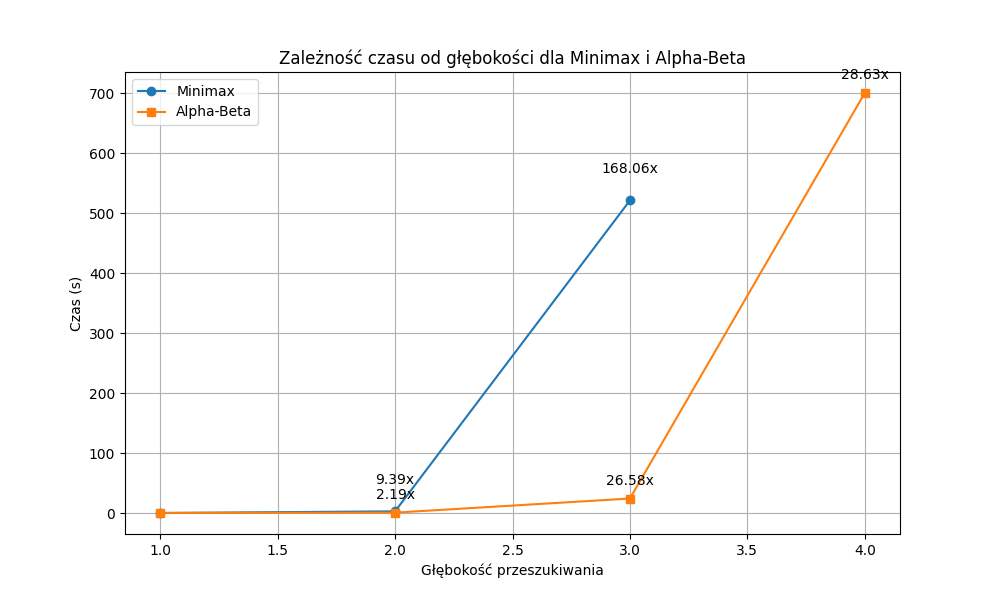
\includegraphics[width=0.8\textwidth]{images/time-depth.png} 
    \caption{Wykres prezentujący wzrost czasu wykonania wraz ze wzrostem głębokości}
\end{figure}
Jak widać na wykresie powyżej, 
czas wykonywania dla algorymu minmax rósł wykładniczo wraz ze wzrostem głębokości.
Już dla głębokośc 3, czas wyszukiwania był 168 razy większy niż dla głębokości 2.
Jeśli chodzi o algorytm \textit{Alphabeta}, to 
rósł on trochę wolniej, jednak już dla głębokości 3
osiągnął on dużą wartość.


\subsection{Przykładowy przebieg gry}
Funkcja main zaczynająca gre wygląda następująco:
\begin{lstlisting}
int main() {
    const IPawnHeuristic &distance = ManhattanDistance();
    const IBoardEvaluator &movePotentialEvaluator =
        MovePotentialEvaluator(distance);
    const IBoardEvaluator &campDistanceEvaluator =
        CampDistanceEvaluator(distance);
    AlphaBetaPlayer player1(campDistanceEvaluator, 2);
    AlphaBetaPlayer player2(campDistanceEvaluator, 2);

    try {
        auto start = chrono::high_resolution_clock::now();

        Halma h(&player1, &player2);
        int visited = h.playGame();

        auto end = chrono::high_resolution_clock::now();
        std::chrono::duration<double> elapsed_seconds = end - start;

        std::cout << "\nVisited a total of: " << visited << " nodes";
        std::cout << "\nCalulation time: " << elapsed_seconds.count()
                  << " seconds";

    } catch (const exception &ex) {
        cerr << "An error occurred: " << ex.what() << endl;
    }
}
\end{lstlisting}


\begin{figure}[H]
    \centering
    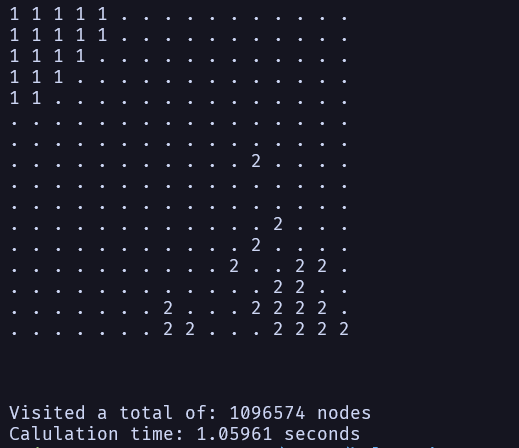
\includegraphics[width=0.8\textwidth]{images/result.png} 
    \caption{Przykładowy wynik gry}
\end{figure}
Zdjęcie powyżej prezentuje przykładowy wynik gry. 
Zaprezentowana jest plansza, liczba odwiedzonych 
węzłów oraz czas wykonania. 










\end{document}